\section{Mechanical Models II}
\label{MechModelsII:sec}

This section provides additional material on building basic
multibody-type mechanical models.

\subsection{Simulation control properties}

Both \javaclass[artisynth.core.workspace]{RootModel} and
\javaclass[artisynth.core.mechmodels]{MechModel} contain properties
that control the simulation behavior. One of the most important of
these is {\tt maxStepSize}. By default, simulation proceeds using the
{\tt maxStepSize} value defined for the root model. A {\tt MechModel}
(or any other type of {\tt Model}) contained in the root model's {\tt
models} list may also request a smaller step size by specifying a
smaller value for its own {\tt maxStepSize} property.  For all models,
the {\tt maxStepSize} may be set and queried using
%
\begin{lstlisting}[]
  void setMaxStepSize (double maxh);
  double getMaxStepSize();
\end{lstlisting}
%

Another important simulation property is {\tt integrator} in {\tt
MechModel}, which determines the type of integrator used for the
physics simulation. The value type of this property is the enumerated
type {\tt MechSystemSolver.Integrator}, for which the following values
are currently defined:

\begin{description}

\item[ForwardEuler]\mbox{}

First order forward Euler integrator. Unstable for stiff systems.

\item[SymplecticEuler]\mbox{}

First order symplectic Euler integrator, more energy conserving
that forward Euler. Unstable for stiff systems.

\item[RungeKutta4]\mbox{}

Fourth order Runge-Kutta integrator, quite accurate but also unstable
for stiff systems.

\item[ConstrainedBackwardEuler]\mbox{}

First order backward order integrator. Generally stable for stiff systems.

\item[Trapezoidal]\mbox{}

Second order trapezoidal integrator. Generally stable for stiff
systems, but slightly less so than {\tt ConstrainedBackwardEuler}.

\end{description}

The term ``Unstable for stiff systems'' means that the integrator is
likely to go unstable in the presence of ``stiff'' systems, which
typically include systems containing finite element models, unless the
simulation step size is set to an extremely small value.  The default
value for {\tt integrator} is {\tt ConstrainedBackwardEuler}.

\begin{sideblock}
Stiff systems tend to arise in models containing interconnected
deformable elements, for which the step size should not exceed the
propagation time across the smallest element, an effect known as the
Courant-Friedrichs-Lewy (CFL) condition. Larger stiffness and damping
values decrease the propagation time and hence the allowable step
size.
\end{sideblock}

Another {\tt MechModel} simulation property is {\tt stabilization},
which controls the stabilization method used to correct drift from
position constraints and correct interpenetrations due to collisions.
The value type of this property value is the enumerated type {\tt
MechSystemSolver.PosStabilization}, which presently has two values:

\begin{description}

\item[GlobalMass]\mbox{}

Uses only a diagonal mass matrix for the MLCP that is solved to
determine the position corrections. This is the default method.

\item[GlobalStiffness]\mbox{}

Uses a stiffness-corrected mass matrix for the MLCP that is solved to
determine the position corrections. Slower than {\tt GlobalMass}, but
more likely to produce stable results, particularly for
problems involving FEM collisions.

\end{description}

\subsection{Units}
\label{sec:mechii:units}

ArtiSynth is primarily ``unitless'', in the sense that it does not
define default units for the fundamental physical quantities of time,
length, and mass. Although time is
generally understood to be in seconds, and often declared as such in
method arguments and return values, there is no hard requirement that
it be interpreted as seconds. There are no assumptions at all
regarding length and mass. Some components may have default parameter
values that reflect a particular choice of units, such as {\tt
MechModel}'s default gravity value of $(0, 0, -9.8)^T$, which is
associated with the MKS system, but these values can always be
overridden by the application.

Nevertheless, it is important, and up to the application developer to
ensure, that units be {\it consistent}. For example, if one decides to
switch length units from meters to centimeters (a common choice),
then all units involving length will have to be scaled appropriately.
For example, density, whose fundamental units are $m/d^3$, where $m$ is mass and
$d$ is distance, needs to be scaled by $1/100^3$, or $0.000001$, when
converting from meters to centimeters.

Table \ref{Units:tab} lists a number of common physical quantities
used in ArtiSynth, along with their associated fundamental units.

\begin{table}
\begin{center}
\begin{tabular}{|lll|}
\hline
unit & fundamental units & \\
\hline
time                    & $t$ & \\
distance                & $d$ & \\
mass                    & $m$ & \\
velocity                & $d/t$ & \\
acceleration            & $d/t^2$ & \\
force                   & $m d/t^2$ & \\
work/energy             & $m d^2/t^2$& \\
torque                  & $m d^2/t^2$ & same as energy (somewhat counterintuitive)\\
angular velocity        & $1/t$ & \\
angular acceleration    & $1/t^2$ & \\
rotational inertia      & $m d^2$ & \\
pressure                & $m/(d t^2)$ & \\
Young's modulus         & $m/(d t^2)$ & \\
Poisson's ratio         & 1 & no units; it is a ratio \\
density                 & $m/d^3$ & \\
linear stiffness        & $m/t^2$ & \\
linear damping          & $m/t$ & \\
rotary stiffness        & $m d^2/t^2$ & same as torque \\
rotary damping          & $m d^2/t$ & \\
mass damping            & $1/t$ & used in FemModel \\
stiffness damping       & $t$ & used in FemModel \\
\hline
\end{tabular}
\end{center}
\caption{Physical quantities and their representation in terms of the
fundamental units of mass ($m$), distance ($d$), and time ($t$).}
\label{Units:tab}
\end{table}

\subsubsection{Scaling units}

For convenience, many ArtiSynth components, including {\tt MechModel},
implement the interface
\javaclass[artisynth.core.util]{ScalableUnits}, which
provides the following methods for scaling mass and distance units:
%
\begin{lstlisting}[]
  scaleDistance (s);    // scale distance units by s
  scaleMass (s);        // scale mass units by s
\end{lstlisting}
%
A call to one of these methods should cause all physical quantities
within the component (and its descendants) to be
scaled as required by the fundamental unit relationships
as shown in Table \ref{Units:tab}.

Converting a {\tt MechModel} from meters to centimeters can therefore be
easily done by calling 
%
\begin{lstlisting}[]
   mech.scaleDistance (100);
\end{lstlisting}
%
As an example, adding the following code to the end of the {\tt build()}
method in {\tt RigidBodySpring} (Section \ref{RigidBodySpringExample:sec})
%
\begin{lstlisting}[]
   System.out.println ("length=" + spring.getLength());
   System.out.println ("density=" + box.getDensity());
   System.out.println ("gravity=" + mech.getGravity());
   mech.scaleDistance (100);
   System.out.println ("");
   System.out.println ("scaled length=" + spring.getLength());
   System.out.println ("scaled density=" + box.getDensity());
   System.out.println ("scaled gravity=" + mech.getGravity());
\end{lstlisting}
%
will scale the distance units by 100 and print the values of various
quantities before and after scaling. The resulting output is:
%
\begin{lstlisting}[]
   length=0.5
   density=20.0
   gravity=0.0 0.0 -9.8

   scaled length=50.0
   scaled density=2.0E-5
   scaled gravity=0.0 0.0 -980.0
\end{lstlisting}
%

\begin{sideblock}
It is important not to confuse scaling units with scaling the actual
geometry or mass. Scaling units should change all physical
quantities so that the simulated behavior of the model remains
unchanged.  If the distance-scaled version of {\tt RigidBodySpring}
shown above is run, it should behave exactly the same as the
non-scaled version.
\end{sideblock}

%\subsection{Multi-point springs}
%OPTIONAL
%\subsubsection{Operation}
%\subsubsection{Example: A single multi-point spring}

%\begin{figure}[ht]
%\begin{center}
%\iflatexml
% 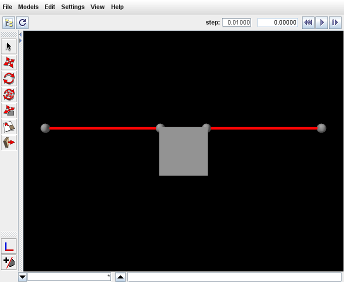
\includegraphics[]{images/MultiPointSpring}
%\else
% 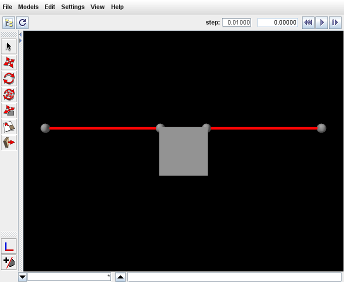
\includegraphics[width=3.75in]{images/MultiPointSpring}
%\fi
%\end{center}
%\caption{MultiPointSpring model loaded into ArtiSynth.}
%\label{MultiPointSpring:fig}
%\end{figure}
%
%A simple model showing a multi-point spring is defined in
%%
%\begin{verbatim}
%  artisynth.demos.tutorial.MultiPointSpring
%\end{verbatim}
%

% MultiPointSpring

\subsection{Point-to-point muscles}
\label{PointToPointMuscles:sec}

Point-to-point muscles are a simple type of component in biomechanical
models that provide muscle-activated forces acting along a line
between two points. ArtiSynth provides this through
\javaclass[artisynth.core.mechmodels]{Muscle}, which is a subclass of
\javaclass[artisynth.core.mechmodels]{AxialSpring} that generates an
active muscle force in response to its {\tt
excitation} property. The excitation property can be set and queried
using the methods
%
\begin{lstlisting}[]
   setExcitation (double a);
   double getExcitation();
\end{lstlisting}
%

\subsubsection{Muscle materials}

As with {\tt AxialSpring}s, {\tt Muscle} components use an
\javaclass[artisynth.core.materials]{AxialMaterial} to compute the
applied force $f (l, \dot l, a)$ in response to the muscle's length
$l$, length velocity $\dot l$, and excitation signal $a$.  Usually the
force is the sum of a {\it passive} component plus an {\it active}
component that arises in response to the excitation signal.

The default {\tt AxialMaterial} for a {\tt Muscle} is
\javaclass[artisynth.core.materials]{SimpleAxialMuscle},
which is essentially an activated version of 
\javaclass[artisynth.core.materials]{LinearAxialMaterial}
and 
which computes a simple force according to
%
\begin{equation}
f(l, \dot l) = k (l-l_0) + d \dot l + m_f a
\end{equation}
%
where $k$ and $d$ are stiffness and damping terms, $a$ is the
excitation value, and $m_f$ is the maximum excitation force.
$k$, $d$ and $m_f$ are exposed through the properties {\tt
stiffness}, {\tt damping}, and {\tt maxForce}.

More complex muscle materials are typically used for biomechanical
modeling applications, generally with non-linear passive terms and
active terms that depend on the muscle length $l$.  Some of those
available in ArtiSynth include
\javaclass[artisynth.core.materials]{ConstantAxialMuscle},
\javaclass[artisynth.core.materials]{BlemkerAxialMuscle},
\javaclass[artisynth.core.materials]{PaiAxialMuscle}, and
\javaclass[artisynth.core.materials]{PeckAxialMuscle}.

% LATER: describe muscles in more detail

\subsubsection{Example: Muscle attached to a rigid body}
\label{SimpleMuscleExample:sec}

\begin{figure}[ht]
\begin{center}
\iflatexml
 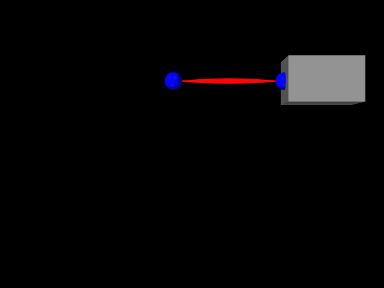
\includegraphics[]{images/SimpleMuscle}
\else
 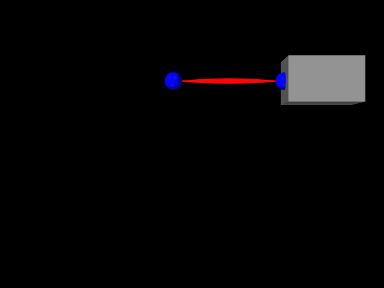
\includegraphics[width=3.75in]{images/SimpleMuscle}
\fi
\end{center}
\caption{SimpleMuscle model loaded into ArtiSynth.}
\label{SimpleMuscle:fig}
\end{figure}

A simple model showing a single muscle connected to a rigid
body is defined in
%
\begin{verbatim}
  artisynth.demos.tutorial.SimpleMuscle
\end{verbatim}
%

This model is identical to {\tt RigidBodySpring} described in Section
\ref{RigidBodySpringExample:sec}, except that the code to create
the spring is replaced with code to create a muscle
with a {\tt SimpleAxialMuscle} material:
%
\begin{lstlisting}[]
      // create the muscle:      
      muscle = new Muscle ("mus", /*restLength=*/0);
      muscle.setPoints (p1, mkr);
      muscle.setMaterial (
         new SimpleAxialMuscle (/*stiffness=*/20, /*damping=*/10, /*maxf=*/10));
\end{lstlisting}
%
Also, so that the muscle renders differently, the rendering style
for lines is set to {\tt ELLIPSOID} instead of {\tt CYLINDER}:
%
\begin{lstlisting}[]
      RenderProps.setLineStyle (r, RenderProps.LineStyle.ELLIPSOID);
\end{lstlisting}
%

To run this example in ArtiSynth, select {\sf All demos > tutorial >
SimpleMuscle} from the {\sf Models} menu. The model should load and
initially appear as in Figure \ref{SimpleMuscle:fig}.  Running the
model (Section \ref{LoadingAndRunning:sec}) will cause the box to fall
and sway under gravity. To see the effect of the {\tt excitation}
property, select the muscle in the viewer and then choose {\sf Edit
properties ...} from the right-click context menu.  This will open an
editing panel that allows the muscle's properties to be adjusted
interactively. Adjusting the {\tt excitation} property using the
adjacent slider will cause the muscle force to vary.

% SimpleMuscle

% LATER \subsubsection{Multi-point muscles}

% LATER \subsection{Mesh components}
%OPTIONAL 
% LATER \subsubsection{Fixed meshes}
% LATER \subsubsection{Simple mesh example}

% SimpleMesh

% LATER \subsubsection{Skinned meshes}
% LATER \subsubsection{Simple skinned mesh example}

% SimpleSkinnedMesh

\subsection{Collision Handling}

Collision handling in ArtiSynth is implemented by a collision
handling mechanism build into {\tt MechModel}. Collisions are
disabled by default, but can be enabled between rigid and deformable
bodies (finite element models in particular), and more generally
between any body that implements the interface 
\javaclass[artisynth.core.mechmodels]{Collidable}.

%\subsubsection{Collidable bodies}

\subsubsection{Enabling collisions in code}

Collisions can be enabled as either a default behavior between all
bodies, a default behavior between certain {\it types} of
bodies, or a specific behavior between individual pairs of bodies.

The default collision behavior between all collidables can be
controlled using two equivalent methods:
%
\begin{lstlisting}[]
  setDefaultCollisionBehavior (enabled, mu);
  setDefaultCollisionBehavior (behavior);
\end{lstlisting}
%
where {\tt enabled} is {\tt true} or {\tt false} depending on whether
collisions are enabled, {\tt mu} is the coefficient of Coulomb (or
dry) friction, and {\tt behavior} is a
\javaclass[artisynth.core.mechmodels]{CollisionBehavior} object that
specifies both {\it enabled} and {\it mu}. The {\tt mu} value is
ignored if {\tt enabled} is {\tt false}.  In addition, collisions can
be controlled for specific {\it types} of collidables using
%
\begin{lstlisting}[]
  setDefaultCollisionBehavior (typeA, typeB, enabled, mu);
  setDefaultCollisionBehavior (typeA, typeB, behavior);
\end{lstlisting}
%
where {\tt typeA} and {\tt typeB} should be either {\tt
Collidable.RigidBody} or {\tt Collidable.Deformable}.  In addition,\\
{\tt Collidable.Deformable} can be paired with {\tt Collidable.Self} to
enable/disable self-collisions between deformable objects.

A call to one of the {\tt setDefaultCollisionBehavior()} methods will
override the effects of previous calls. So for instance, the code
sequence
%
\begin{lstlisting}[]
  setDefaultCollisionBehvaior (true, 0);
  setDefaultCollisionBehvaior (
    Collidable.Deformable, Collidable.RigidBody, false, 0);
  setDefaultCollisionBehavior (true, 0.2);
\end{lstlisting}
%
will initially enable collisions between all bodies with a friction
coefficient of 0, then {\it disable} collisions between deformable and
rigid bodies, and finally re-enable collisions between all bodies with
a friction coefficient of 0.2.

The default collision behavior between any pair of body types can
be queried using
%
\begin{lstlisting}[]
  CollisionBehavior getDefaultCollisionBehavior (typeA, typeB);
\end{lstlisting}
%

In addition to default behaviors, collisions between individual
collidables can be controlled and queried using
%
\begin{lstlisting}[]
  setCollisionBehavior (collidableA, collidableB, enabled, mu);
  setCollisionBehavior (collidableA, collidableB, behavior);
  getCollisionBehavior (collidableA, collidableB);
\end{lstlisting}
%
where {\tt collidableA} and {\tt collidableB} are individual
collidable components such as rigid bodies or FEM models.  The effects
of {\tt setCollisionBehavior()} methods are {\it not} invalidated by
subsequent calls to {\tt setDefaultCollisionBehavior()} methods.

\begin{sideblock}
It is usually necessary to ensure that collisions are {\it disabled}
between adjacent bodies connected by joints, since otherwise these
would be forced into a state of permanent collision.
\end{sideblock}

\subsubsection{Example: Collision with a plane}

\begin{figure}[ht]
\begin{center}
\iflatexml
 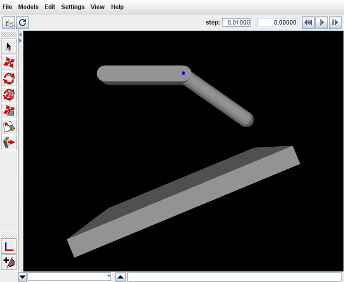
\includegraphics[]{images/JointedCollide}
\else
 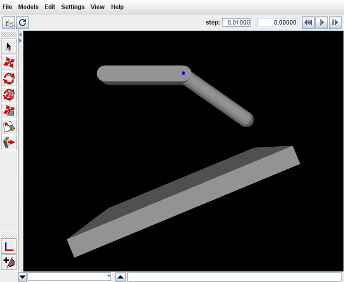
\includegraphics[width=3.75in]{images/JointedCollide}
\fi
\end{center}
\caption{JointedCollide model loaded into ArtiSynth.}
\label{JointedCollide:fig}
\end{figure}

A simple model illustrating collision between two jointed rigid bodies
and a plane is defined in
%
\begin{verbatim}
  artisynth.demos.tutorial.JointedCollide
\end{verbatim}
%

This model is simply a subclass of {\tt RigidBodyJoint} that
overrides the {\tt build()} method 
to add an inclined plane and enable collisions between it and
the two connected bodies:
%
\lstset{numbers=left}
\begin{lstlisting}[]
   public void build (String[] args) {

      super.build (args);

      bodyB.setDynamic (true);  // allow bodyB to fall freely

      // create and add the inclined plane
      RigidBody base = RigidBody.createBox ("base", 25, 25, 2, 0.2);
      base.setPose (new RigidTransform3d (5, 0, 0, 0, 1, 0, -Math.PI/8));
      base.setDynamic (false);
      mech.addRigidBody (base);

      // turn on collisions
      mech.setDefaultCollisionBehavior (true, 0.20);
      mech.setCollisionBehavior (bodyA, bodyB, false);
   }
\end{lstlisting}
\lstset{numbers=none}

The superclass {\tt build()} method called at line 3 creates
everything contained in {\tt RigidBodyJoint}. The remaining code then
alters that model: {\tt bodyB} is set to be dynamic (line 5) so that
it will fall freely, and an inclined plane is created from a thin box
that is translated and rotated and then set to be be non-dynamic
(lines 8-11).  Finally, collisions are enabled by setting the default
collision behavior (line 14), and then specifically disabling
collisions between {\tt bodyA} and {\tt bodyB} (line 15). As indicated
above, the latter step is necessary because the joint would otherwise
keep the two bodies in a permanent state of collision.

To run this example in ArtiSynth, select {\sf All demos > tutorial >
JointedCollide} from the {\sf Models} menu. The model should load and
initially appear as in Figure \ref{JointedCollide:fig}.  Running
the model (Section \ref{LoadingAndRunning:sec}) will
cause the jointed assembly to collide with and slide off the inclined
plane.

\subsubsection{Implementation and limitations}

The ArtiSynth collision mechanism works by finding intersections
between the surface meshes of each collidable object.  These surface
meshes must (at present) be triangular, closed, and manifold.
A bounding-box 
hierarchy is used to determine if any two surfaces meshes
intersect. If they do, then a tracing algorithm
is used to compute all the intersection contours
between the two meshes as shown in Figure~\ref{Collision:fig}.

\begin{figure}[ht]
\begin{center}
        \begin{tabular}{ccc}
        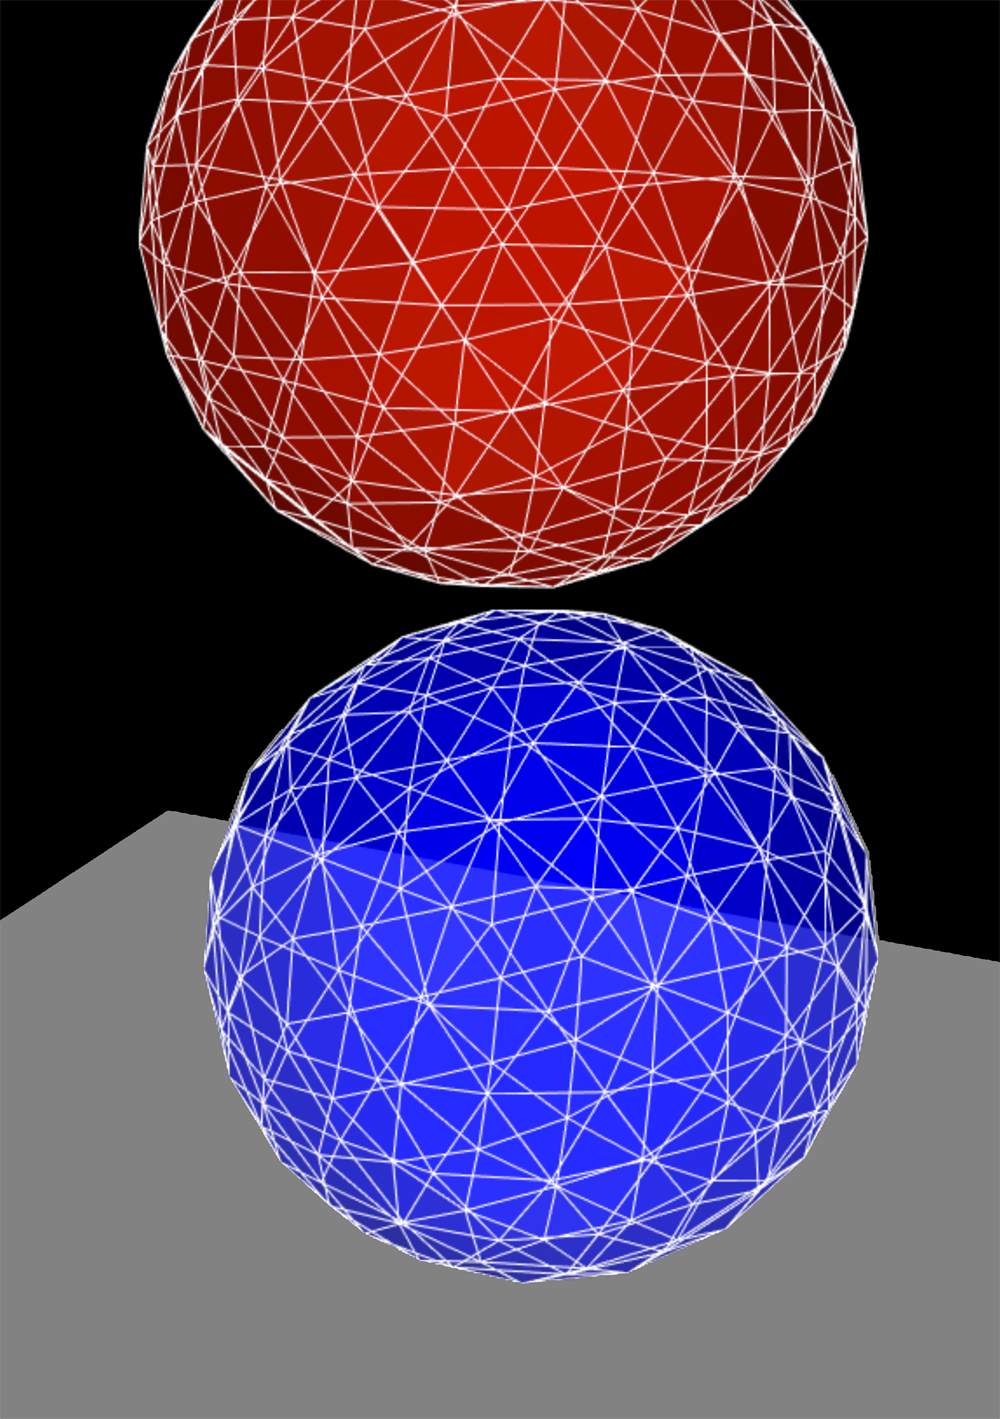
\includegraphics[width=0.31\textwidth]{images/femCollide1} &
        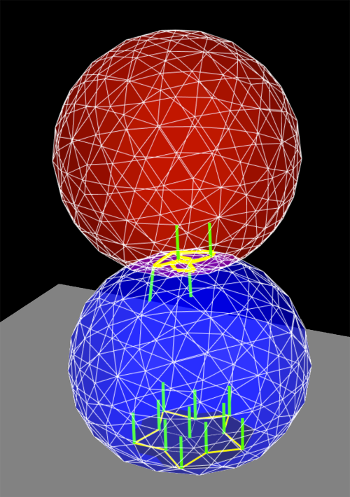
\includegraphics[width=0.31\textwidth]{images/femCollide2} &
        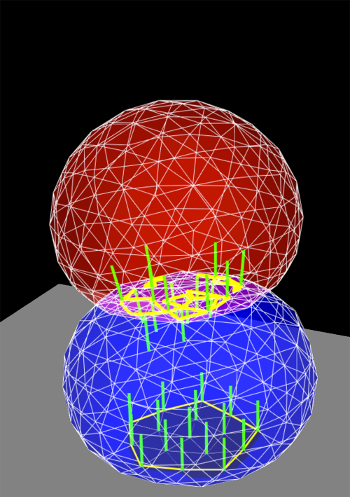
\includegraphics[width=0.31\textwidth]{images/femCollide3}\\
%       \end{tabular}
%       \begin{tabular}{p{1.2cm}p{3.5cm}p{3.5cm}p{3.5cm}} 
         \large  $\mathrm{t}=0$s & \large $\mathrm{t}=0.25$s & \large $\mathrm{t}=0.5$s         
        \end{tabular}
\end{center}
\caption{Time sequence of contact handling between two deformable models 
falling under gravity, 
showing the intersection contours
(yellow) and the contact normals (green lines).}
\label{Collision:fig}
\end{figure}

Determining the intersection contour allows us to create a set of
constraints for correcting the interpenetration and preventing
interpenetrating velocities.  For rigid bodies, this is done by
fitting a plane to each contour, projecting the contour onto this
plane, and then sampling the vertices of the projection's 2D convex
hull to create individual contact points, with the contact normal set
from the normal of the plane. For deformable FEM models, the
intersection contour is used to locate all the interpenetrating nodes,
and then collision constraints are established between each node and
the nearest triangular face of the opposing surface.

Because ArtiSynth currently uses static collision detection, it is
possible for objects that are fast enough or thin enough to completely
pass through each other in one simulation step. This means that for
thin objects, it is important to keep the step size small enough to
prevent such undetected interpenetration.

ArtiSynth also uses a ``box'' friction approximation
\cite{Lacoursiere07} to compute dry friction, instead of the
polyhedralized friction cones common in the multibody dynamics
literature \cite{AnitescuPotra2002,PotraEtAlTrapezoidal2006}.  This
allows for a less expensive and more robust computation at the expense
of some accuracy.

Another issue is that ArtiSynth's attempt to separate colliding bodies
at the end of each time step may cause a jittering behavior around the
colliding area, as the surface collides, separates, and re-collides.
This can usually be stabilized by maintaining a certain
interpenetration distance during contact. This distance is controlled
by the {\tt MechModel} property {\tt penetrationTol}.  ArtiSynth
attempts to compute a suitable default value for this property, but
for some applications it may be necessary to control the value
explicitly using the {\tt MechModel} methods
%
\begin{lstlisting}[]
   setInterpenetrationTol (double dist);
   double getInterpenetrationTol();
\end{lstlisting}
%

Other aspects of collision handling can be adjusted by directly
setting properties of the {\tt MechModel}'s collision manager, which
can be accessed graphically via the navigation panel, or in code using
\javamethod*[artisynth.core.mechmodels.MechModel]{getCollisionManager()}.

One of these properties is {\tt collisionPointTol}, which for
collisions between rigid bodies specifies a minimum distance between
contact points and therefore can be used to reduce the number of
contact constraints and improve computation time.

% LATER: \subsubsection{Contact rendering}

% LATER \subsection{Moving non-dynamic components}

% LATER \subsection{General component arrangements}
% LATER \label{GeneralArrangements:sec}

% LATER \subsubsection{Component lists}

% LATER \subsubsection{General arrangement example}

% LATER NetDemo

% LATER \subsubsection{Legacy containers in MechModel}

\subsection{Render properties}
\label{RenderProperties:sec}

All ArtiSynth components that are renderable maintain a property {\tt
renderProps}, which stores a
\javaclass[maspack.render]{RenderProps} object that contains a number
of subproperties used to control an object's rendered appearance.

In code, the {\tt renderProps} property for an object can be set or
queried using the methods
%
\begin{lstlisting}[]
  setRenderProps (RenderProps props); // set render properties
  RenderProps getRenderProps();       // get render properties (read-only)
\end{lstlisting}
%
Render properties can also be set in the GUI by selecting one or more
components and the choosing {\sf Set render props ...}  in the
right-click context menu. More details on setting render properties
through the GUI can be found in the section ``Render properties'' in the
\href{../uiguide/uiguide.html}{
ArtiSynth User Interface Guide}.

For many components, the default value of {\tt renderProps} is {\tt
null}; i.e., no {\tt RenderProps} object is assigned by default and
render properties are instead inherited from ancestor components
further up the hierarchy. The reason for this is because {\tt
RenderProps} objects are fairly large (many kilobytes), and so
assigning a unique one to every component could consume too much
memory. Even when a {\tt RenderProps} object is assigned, most of its
properties are inherited by default, and so only those properties
which are explicitly set will differ from those specified in ancestor
components.

\subsubsection{Render property taxonomy}

In general, the properties in {\tt RenderProps} are used to control
the color, size, style, and resolution of the three primary rendering
primitives: faces, lines, and points. Table \ref{RenderProps:tab}
contains a complete list. Values for the {\tt shading}, {\tt
faceStyle}, {\tt lineStyle} and {\tt pointStyle} properties are
defined using the enumerated types {\tt RenderProps.Shading}, {\tt
RenderProps.Faces}, {\tt RenderProps.LineStyle}, and {\tt
RenderProps.PointStyle}.  Colors are specified using {\tt
java.awt.Color}.

\begin{table}
\begin{center}
\begin{tabular}{|lll|}
\hline property & purpose & usual default value \\ \hline
%Generic properties:
visible & whether or not the component is visible & {\tt true} \\
alpha & transparency for polygonal faces (range 0 to 1) & 1 (opaque) \\
shading & polygon shading: ({\tt FLAT}, {\tt GOURARD}, {\tt PHONG}) & {\tt FLAT}\\
shininess & shininess parameter for polygons (range 0 to 32) & 32 \\
%Face related properties &
\hline
faceStyle &
which polygonal faces are drawn ({\tt FRONT}, {\tt BACK},
{\tt FRONT\_AND\_BACK}, {\tt NONE}) & {\tt FRONT} \\
faceColor &
color used for drawing faces & {\tt GREY} \\
backColor &
color used for drawing backs of faces. If {\tt null}, {\tt faceColor} is used. &
{\tt null} \\
drawEdges & if true, polygon edges are drawn explicitly & {\tt false} \\
% Edge related properties &
\hline
edgeColor & color for edges & {\tt GREY} \\
edgeWidth & edge width in pixels & 1 \\
% Line related properties &
\hline
lineStyle: &
how lines are drawn ({\tt CYLINDER}, {\tt LINE}, or {\tt ELLIPSOID}) & 
{\tt LINE} \\
lineColor & color for lines & {\tt GREY} \\
lineWidth & width in pixels when {\tt LINE} style is selected & 1 \\
lineRadius & radius when {\tt CYLINDER} or {\tt ELLIPSOID} style is selected &
1 \\
lineSlices &
number of slices used to render {\tt CYLINDER} or {\tt ELLIPSOID} style lines &
32 \\
% Point related properties &
\hline
pointStyle & how points are drawn ({\tt SPHERE} or {\tt POINT}) & {\tt POINT} \\
pointColor & color for points & {\tt GREY} \\
pointSize & point size in pixels when {\tt POINT} style is selected & 1 \\
pointRadius & sphere radius when {\tt SPHERE} style is selected & 1 \\
pointSlices & number of slices used to render {\tt SPHERE} style spheres & 32 \\
\hline
\end{tabular}
\end{center}
\caption{Render properties and their default values.}
\label{RenderProps:tab}
\end{table}

To increase and improve their visibility, both the line and point
primitives are associated with styles ({\tt CYLINDER}, {\tt
ELLIPSOID}, and {\tt SPHERE}) that allow them to be rendered using 3D
surface geometry.

Exactly how a component interprets its render properties is up to the
component (and more specifically, up to the rendering method for that
component).  Not all render properties are relevant to all components,
particularly if the rendering does not use all of the rendering
primitives. For example,
\javaclass[artisynth.core.mechmodels]{Particle} components use only
the point primitives and
\javaclass[artisynth.core.mechmodels]{AxialSpring} components use only
the line primitives. For this reason, some components use subclasses
of {\tt RenderProps}, such as
\javaclass[maspack.render]{PointRenderProps} and
\javaclass[maspack.render]{LineRenderProps}, that expose only a subset
of the available render properties. All renderable components provide
the method
\javamethod[maspack.render.HasRenderProps]{createRenderProps()} that
will create and return a {\tt RenderProps} object suitable for that
component.

\subsubsection{Setting render properties}

When setting render properties, it is important to note that
the value returned by
\javamethod[maspack.render.HasRenderProps]{getRenderProps()} 
should be treated as {\it read-only} and should {\it not}
be used to set property values.
For example, applications should {\it not} do the
following:
\begin{lstlisting}[]
   particle.getRenderProps().setPointColor (Color.BLUE);
\end{lstlisting}
%
This can cause problems for two reasons. First, {\tt getRenderProps()}
will return {\tt null} if the object does not currently have a {\tt
RenderProps} object. Second, because {\tt RenderProps} objects are
large, ArtiSynth may try to share them between components, and so by
setting them for one component, the application my inadvertently set
them for other components as well.

Instead, {\tt RenderProps} provides a static method for each property
that can be used to set that property's value for a specific
component.  For example, the correct way to set {\tt pointColor} is
%
\begin{lstlisting}[]
   RenderProps.setPointColor (particle, Color.BLUE);
\end{lstlisting}
%

One can also set render properties by calling
\javamethod*[maspack.render.HasRenderProps]{setRenderProps()} with a
predefined {\tt RenderProps} object as an argument. This is useful for
setting a large number of properties at once:
%
\begin{lstlisting}[]
   RenderProps props = new RenderProps();
   props.setPointColor (Color.BLUE);
   props.setPointRadius (2);
   props.setPointStyle (RenderProps.PointStyle.SPHERE);

   ...

   particle.setRenderProps (props);
\end{lstlisting}

\begin{sideblock}
Note that even though components may use a subclass of {\tt
RenderProps} internally, one can always use the base {\tt RenderProps}
class to set values; properties which are not relevant to the
component will simply be ignored.
\end{sideblock}

Finally, as mentioned above, render properties are inherited.  Values
set high in the component hierarchy will be inherited by descendant
components, unless those descendants (or intermediate components)
explicitly set overriding values.  For example, a {\tt MechModel}
maintains its own {\tt RenderProps} (and which is never null). Setting
its {\tt pointColor} property to {\tt RED} will cause {\it all}
point-related components within that {\tt MechModel} to be rendered as
red {\it except} for components that set their {\tt pointColor} to a
different property.

There are typically three levels in a {\tt MechModel} component
hierarchy at which render properties can be set:

\begin{itemize}

\item The {\tt MechModel} itself;

\item Lists containing components;

\item Individual components.

\end{itemize}

For example, consider the following code:
%
\begin{lstlisting}[]
   MechModel mech = new MechModel ("mech");

   Particle p1 = new Particle (/*name=*/null, 2, 0, 0, 0);
   Particle p2 = new Particle (/*name=*/null, 2, 1, 0, 0);
   Particle p3 = new Particle (/*name=*/null, 2, 1, 1, 0);

   mech.addParticle (p1);
   mech.addParticle (p2);
   mech.addParticle (p3);

   RenderProps.setPointColor (mech, Color.BLUE);
   RenderProps.setPointColor (mech.particles(), Color.GREEN);
   RenderProps.setPointColor (p3, Color.RED);   
\end{lstlisting}
%
Setting the {\tt MechModel} render property {\tt pointColor} to {\tt
BLUE} will cause all point-related items to be rendered blue by
default. Setting the {\tt pointColor} render property for the particle
list (returned by {\tt mech.particles()}) will override this and cause
all particles in the list to be rendered green by default. Lastly,
setting {\tt pointColor} for {\tt p3} will cause it to be rendered as
red.

%

% LATER \subsection{Transforming Geometry}

% LATER \subsubsection{The TransformableGeometry interface}
